\documentclass[10pt, margin = -0.1172cm]{standalone}
\usepackage{tikz}
\usetikzlibrary{calc}
\usetikzlibrary{matrix}
\usepackage{pifont}
\usepackage{mathtools}

\definecolor{pink}{RGB}{237,16,118}
\definecolor{applegreen}{rgb}{0.55, 0.71, 0.0}
\definecolor{celestialblue}{RGB}{62,146,204}
\definecolor{lila}{RGB}{125,41,221}
% Satellite colors
\definecolor{colormult00}{RGB}{86, 180, 233}%light blue
\definecolor{colormult01}{RGB}{230, 159, 0}%orange
\definecolor{colormult02}{RGB}{204, 121, 167}%lila
\definecolor{colormult03}{RGB}{240, 228, 66}%gelb
\definecolor{colormult04}{RGB}{0, 158, 115}%grün
\definecolor{colormult05}{RGB}{213, 94, 0}%rötliches orange
\definecolor{colormult06}{RGB}{0, 114, 178}%dark blue
\definecolor{colormult07}{RGB}{0,0,0}
% Quantum colors
\definecolor{violet}{HTML}{53257F} %Quantum violet
\definecolor{green}{HTML}{257a7f}%{507F25} %Quantum green
\definecolor{brown}{HTML}{852e29}%{7F3B25} %Quantum brown

% Commands for the notation
\newcommand{\qubt}[1]{\ensuremath{\tau_{#1}}}    % Top qubit for a node in EPR pair with node on the right
\newcommand{\qubb}[1]{\ensuremath{\omega_{#1}}}  % Bottom qubit for a node in EPR pair with node on the left

\newcommand{\spmo}[1]{\ensuremath{o_{#1}}} % State preparation measurement outcome
\newcommand{\gemo}[1]{\ensuremath{m_{#1}}} % GHZ extraction measurement outcome
\newcommand{\gemb}[1]{\ensuremath{\beta_{#1}}} % GHZ extraction measurement basis bit

\newcommand{\yes}[1]{\ding{51}$_{#1}$}
\newcommand{\no}[0]{\ding{55}}

\newcommand{\fourgroup}[0]{\ensuremath{g_{ab}}}    % Symbol for the number of four-groups in \delta_{ab}
\newcommand{\modfourval}[0]{\ensuremath{\delta_{ab} \mod 4}} % Symbol for the mod-four value of \delta_{ab}

\begin{document}
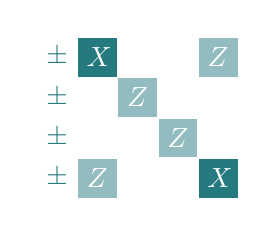
\begin{tikzpicture}
\matrix (M) [
	matrix of nodes,
	minimum width=1cm,
	minimum height=1cm,
	column sep=0mm,
	row sep=0mm,
	nodes={
		draw,
		color = white,
		line width=0.07mm,
		anchor=south,
		align=center,
	},
	row 1/.style={
		nodes={
			minimum height=0.505cm,
		}
	},
	row 2/.style={
		nodes={
			minimum height=0.505cm,
		}
	},
	row 3/.style={
		nodes={
			minimum height=0.505cm,
		}
	},
	row 4/.style={
		nodes={
			minimum height=0.505cm,
		}
	},
	column 1/.style={
		nodes={
			text width=0.27cm,
			minimum width=0.27cm,
		}
	},
	column 2/.style={
		nodes={
			text width=0.27cm,
			minimum width=0.27cm,
		}
	},
	column 3/.style={
		nodes={
			text width=0.27cm,
			minimum width=0.27cm,
		}
	},
	column 4/.style={
		nodes={
			text width=0.27cm,
			minimum width=0.27cm,
		}
	},
	column 5/.style={
		nodes={
			text width=0.27cm,
			minimum width=0.27cm,
		}
	}
]{
|[fill=white!100]|\textcolor{green}{$\pm$}
	&|[fill=green!100]|\textcolor{white}{$X$}
	&|[fill=white!100]|\textcolor{green}{$ $}
	&|[fill=white!100]|\textcolor{green}{$ $}
	&|[fill=green!50]|\textcolor{white}{$Z$}
\\|[fill=white!100]|\textcolor{green}{$\pm$}
	&|[fill=white!100]|\textcolor{green}{$ $}
	&|[fill=green!50]|\textcolor{white}{$Z$}
	&|[fill=white!100]|\textcolor{green}{$ $}
	&|[fill=white!100]|\textcolor{green}{$ $}
\\|[fill=white!100]|\textcolor{green}{$\pm$}
	&|[fill=white!100]|\textcolor{green}{$ $}
	&|[fill=white!100]|\textcolor{green}{$ $}
	&|[fill=green!50]|\textcolor{white}{$Z$}
	&|[fill=white!100]|\textcolor{green}{$ $}
\\|[fill=white!100]|\textcolor{green}{$\pm$}
	&|[fill=green!50]|\textcolor{white}{$Z$}
	&|[fill=white!100]|\textcolor{green}{$ $}
	&|[fill=white!100]|\textcolor{green}{$ $}
	&|[fill=green!100]|\textcolor{white}{$X$}
\\
};
\end{tikzpicture}
\end{document}